%%%%%%%%%%%%%%%%%%%%%%%%%%%%%%%%%%%
\begin{exo}[2][oral]{Lévitation d’une balle de ping-pong}
    Une balle de ping-pong de diamètre $\SI{40}{mm}$ et de masse $\SI{3}{g}$ lévite au dessus d'un sèche-cheveux de diamètre $\SI{5}{cm}$ qui envoie un flux d'air de débit volumique $\SI{0.5}{L.s^{-1}}$. La viscosité cinématique de l'air vaut $\SI{e-5}{m^2.s^{-1}}$. On donne ci-dessous le graphe du coefficient de traînée en fonction du nombre de Reynolds pour une sphère.
    \begin{center}
        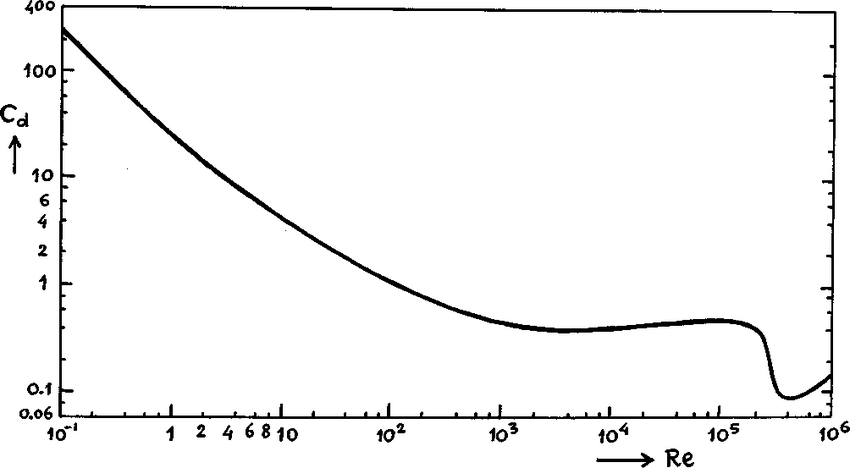
\includegraphics[width=0.6\textwidth]{drag_coeff_sphere.png}
    \end{center}
  Expliquer pourquoi la balle de ping-pong lévite.
  \solution{
  \underline{Méthode de résolution} d'un problème ouvert.
  \begin{itemize}
    \item \underline{S'approprier} : identifier les données, faire un schéma, traduire en langage mathématique.
    \item \underline{Analyser} : choisir un cadre d'étude, décomposer en sous-problèmes simples, procéder par analogie avec un problème connu.
    \item \underline{Réaliser} : vérifier chaque étape, mener les calculs.
    \item \underline{Valider} : relire la solution en recherchant le erreurs, comparer le modèle à la réalité.
    \item \underline{Communiquer} : rédiger de façon organisée, rigoureuse, claire et efficace.
  \end{itemize}
  Appliquons cette méthode ici.
  \begin{itemize}
    \item L'énoncé nous donne deux diamètres $d=40 \mathrm{~mm}$ et $D=5 \mathrm{~cm}$, la masse $m=\SI{50}{g}$, le débit volumique $D_V = \SI{0.5}{L.s^{-1}}$, la viscosité cinématique de l'air $\nu=10^{-5} \mathrm{~m}^2 \cdot \mathrm{s}^{-1}$, et la fonction coefficient de traînée $Cd(\text{Re})$.
    \item La présence de ce graphe suggère qu'on étudie la dynamique visqueuse des fluides newtoniens. La dynamique visqueuse est caractérisée par le nombre de Reynolds $\text{Re}$, tandis que le coefficient de traînée intervient dans la force de traînée $\F$. Pour répondre à la question, on peut décomposer en sous-problèmes :
    évaluer $\text{Re}$, en déduire la valeur de $Cd$ à partir du graphe, évaluer la force de traînée $F$, et la comparer au poids $P$.
    \item On utilise les connaissances de cours.
    \begin{itemize}
      \item
    Nombre de Reynolds $\text{Re} = \frac{UL}{\nu}$ où $U$ est la vitesse caractéristique de l'écoulement, et $L$ la taille typique de l'obstacle. On utilise les données de l'énoncé : $L=d$ est la taille de la balle, tandis que le débit volumique peut s'écrire $D_V = U S = U \frac{\pi D^2}{4}$, où $S$ est la section de l'écoulement. On trouve $U=\SI{}{}$ puis $\text{Re} = $.
    \item On lit ensuite sur le graphe $Cd = $.
    \item On en déduit la force de traînée $F = \frac{1}{2} Cd \rho U s^2$ où $s=\frac{1}{4}\pi d^2$
    est la section de l'obstacle, et $\rho$ la masse volumique de l'air. On peut proposer $\rho \simeq \SI{e3}{kg.m^{-3}}$. On trouve $F = \SI{}{}$.
    \item On compare au poids de la balle $P=mg = \SI{}{}$. On voit que $F>P$, ce qui explique que la balle puisse léviter.
  \end{itemize}
  \end{itemize}
  }
  \end{exo}
  %%%%%%%%%%%%%%%%%%%%%%%%%%%%%%%%%%%